\documentclass{beamer}
\usetheme{CambridgeUS}

\usepackage{amsmath}
\usepackage{amsfonts}
\usepackage{amssymb}
\usepackage{graphicx}
\usepackage{subfig}
\usepackage{listings}
\usepackage{color}

%Title and such
\title{Classification of Grey-scale Images}
\author{Paula Kimmerling}
\date{April 26,2022}

%Code Presets
\definecolor{dkgreen}{rgb}{0,0.6,0.3}
\definecolor{gray}{rgb}{0.5,0.7,0.5}
\definecolor{mauve}{rgb}{0.58,0,0.82}
\lstset{frame=tb,
	language=Python,
	aboveskip=3mm,
	belowskip=3mm,
	showstringspaces=false,
	columns=flexible,
	basicstyle={\small\ttfamily},
	numbers=none,
	numberstyle=\tiny\color{gray},
	keywordstyle=\color{dkgreen},
	commentstyle=\color{mauve},
	stringstyle=\color{red},
	breaklines=true,
	breakatwhitespace=true,
	tabsize=3
}

\begin{document}
	\begin{frame}
		\titlepage
	\end{frame}
	\begin{frame}
		\tableofcontents
	\end{frame}
\section{The Dataset}
%The presentation will cover your choice of dataset; 
	\begin{frame}
		\frametitle{The Dataset}
		\begin{itemize}
			\pause
			\item Wanted to work with image classification, found the MNIST database of handwritten digits.
			\pause
			\item There were 60,000 training samples and 10,000 testing samples already separated.
			\pause
			\item Each sample was a pre-processed 28 x 28 matrix of integers 0 - 255, with 0 indicating no saturation vs 255 full saturation.
		\end{itemize}
	\begin{figure}
		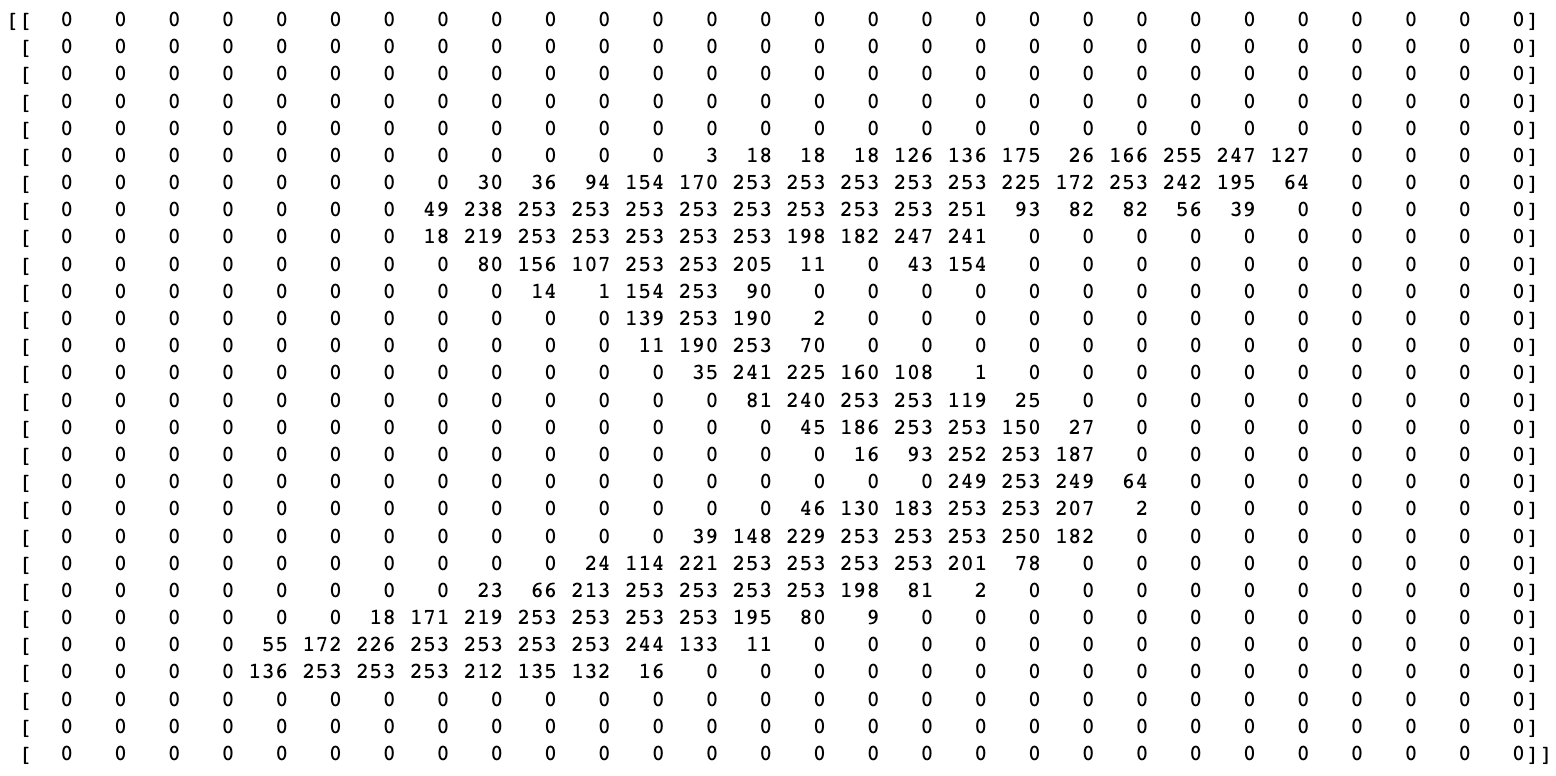
\includegraphics[width=0.5\linewidth]{/Users/paula/Documents/Github/pkimmerling/Neural_Networks/MNIST-5.png}
	\end{figure}
	\end{frame}
\section{Training Choices}
%the choice of output encoding; 
%the choice of cost and activation functions; 
	\begin{frame}
		\frametitle{My Desired Implementation}
		\begin{enumerate}
			\pause
			\item Read in 60,000 matrices and reshape them to be 60,000 row vectors.
			\pause
			\item Encode output data 0-9 as binary (only need 4 outputs):
			$$[0 1 1 1] = 0\cdot2^3 + 1\cdot2^2 +1\cdot2^1 +1\cdot 2^0 = 4+2+1 =7$$
			\pause
			\item Use ensemble cost function.
			\pause
			\item Use LReLU as first activation and logistic as second activation.
			\pause
			\item Use bfgs as the non-linear solver.
			\pause
			\item Read back the binary numbers to integer to compare.
		\end{enumerate}
	\end{frame}
	\begin{frame}[fragile]
		\frametitle{What Actually Happened}
		60,000 samples was too much for my local code. So I used the MLPCLassifier from sci-kit learn which runs faster because it has bits already compiled:
		\begin{lstlisting}
		from sklearn.neural_network import MLPClassifier
		
		clf = MLPClassifier(solver=`lbfgs', activation=`logistic',alpha=regParam,
		hidden_layer_sizes=(k,), random_state=1)
		start = time.time()
		clf.fit(trainX,trainY)
		end = time.time()
		print("Time to train:", end-start)
		\end{lstlisting}
		\texttt{Time to train: 581.859} $\approx 9.7$ minutes
	\end{frame}
\section{Fits}
%the fit to the training data; and the error in predictions for your test samples, which will be different from your training data.
	\begin{frame}[fragile]
		\frametitle{Fit to Train Data}
		It trained to fit the data perfectly in this case, because the `score' attribute of the classifier gives an average percentage accuracy.
		\begin{lstlisting}
		pred = clf.predict(trainX)
		clf.score(trainX,trainY)
		\end{lstlisting}
		\texttt{1.0} = $100$\%\\
		It also didn't do too badly on the testing data:
		\begin{lstlisting}
		pred = clf.predict(testX)
		clf.score(testX,testY)
		\end{lstlisting}
		\texttt{0.8276} = $82.76$\%
	\end{frame}
	\begin{frame}
		\frametitle{Examples of Test Data Outputs}
		\begin{figure}
			\centering
			\subfloat{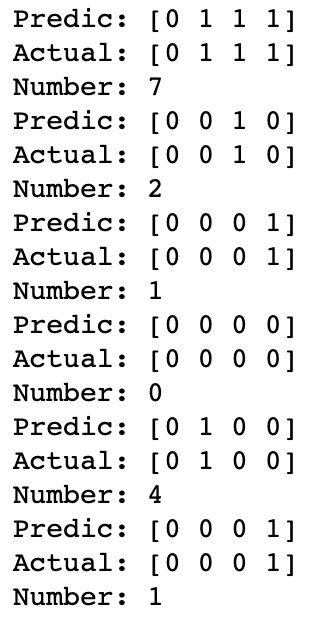
\includegraphics[width=0.3\linewidth]{/Users/paula/Documents/Github/pkimmerling/Neural_Networks/MNISTOut1.png}}
			\subfloat{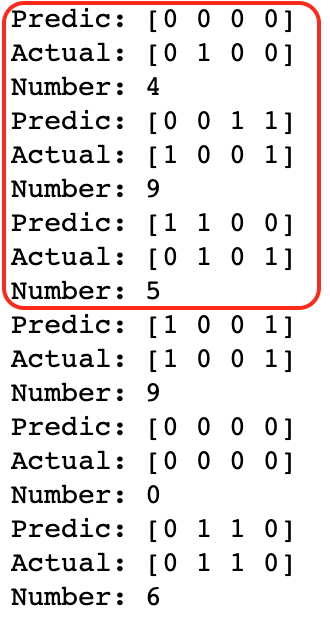
\includegraphics[width=0.3\linewidth]{/Users/paula/Documents/Github/pkimmerling/Neural_Networks/MNISTOut2.png}}
			\subfloat{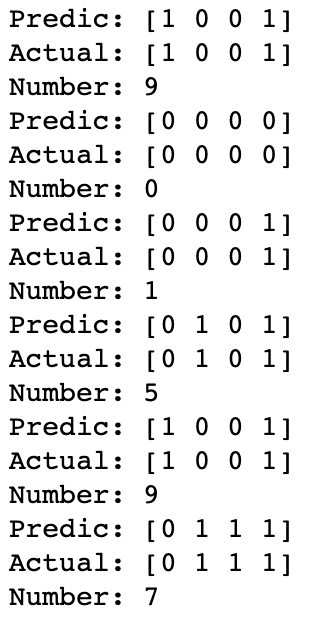
\includegraphics[width=0.3\linewidth]{/Users/paula/Documents/Github/pkimmerling/Neural_Networks/MNISTOut3.png}}
		\end{figure}
	\end{frame}
\end{document}